% Degree process (cumulative count) in MG
%  2x2 figure  
%  [glogal expectaion] [global variance]
%  [local expectation] [local variance]
%
% pmk PNAS3 -x burst_process_mg -g -c BA -n 200 --epoch 10
% pmk PNAS3 -x burst_process_local_mg -g -c BA -n 200 --epoch 100


\begin{figure}[h]
    \centering
    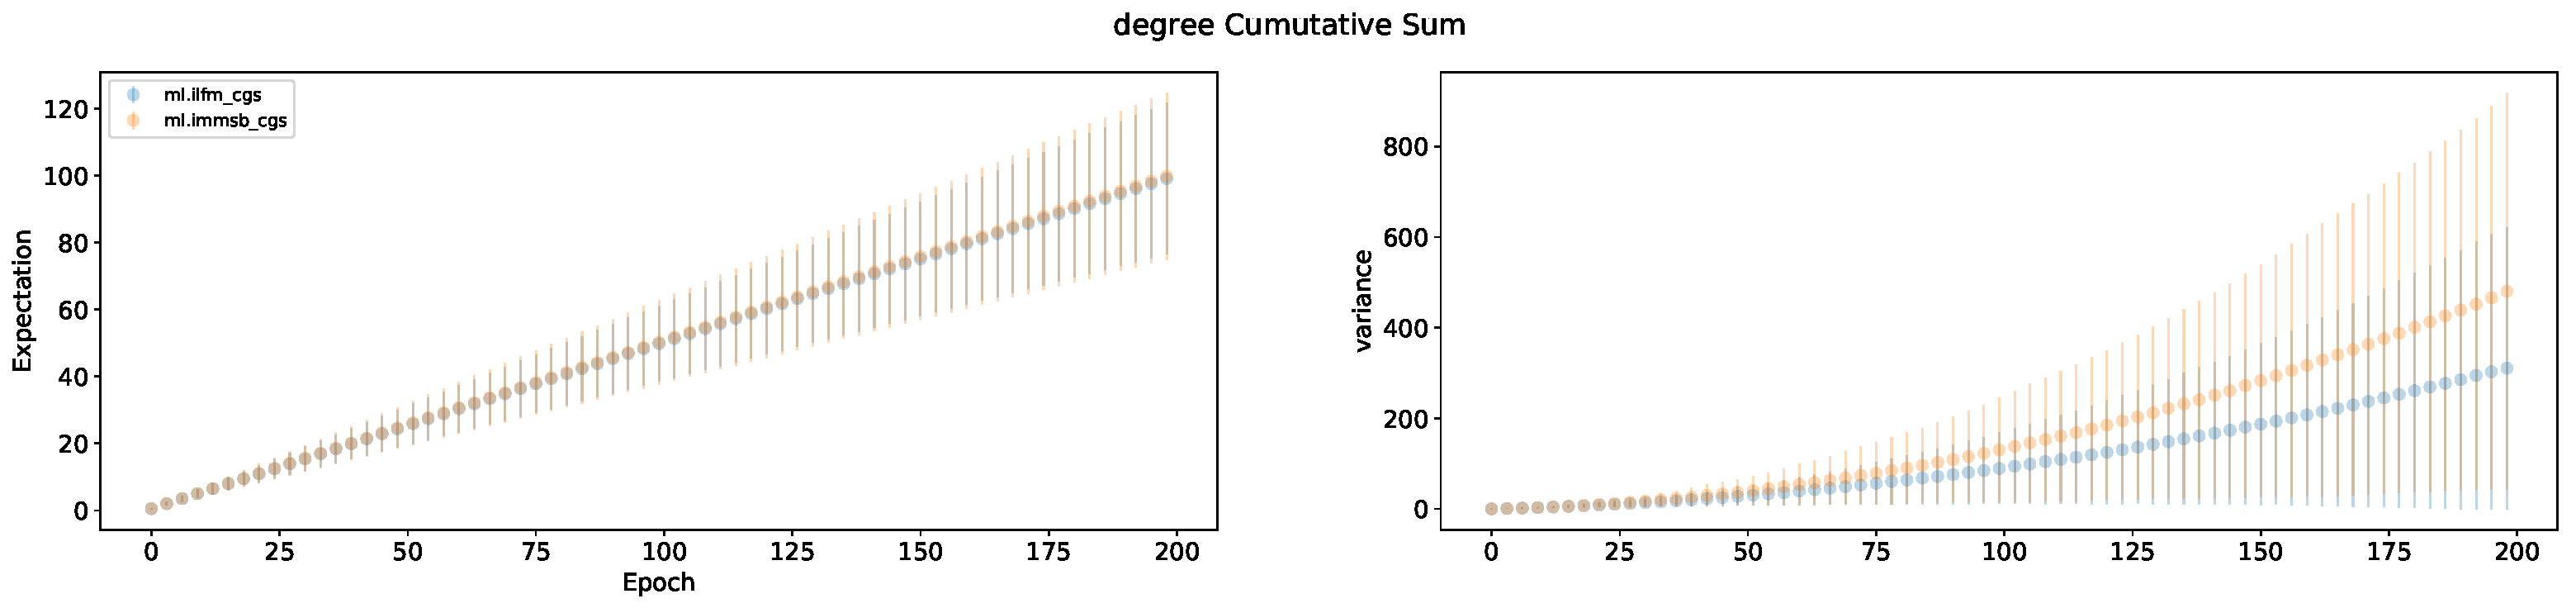
\includegraphics[width=\textwidth, height=6cm]{{{img/0201/BA_burst_process_mg_BA}}}
    \caption {The Left plot is the expectation of the degree count process over the nodes of the network. The right plot is the variance of the degree count process over the nodes of the network. The standard deviation of the curves is the deviation according to each epoch generation.} 
\end{figure}

\begin{figure}[h]
    \centering
    \begin{minipage}{0.99\textwidth}
        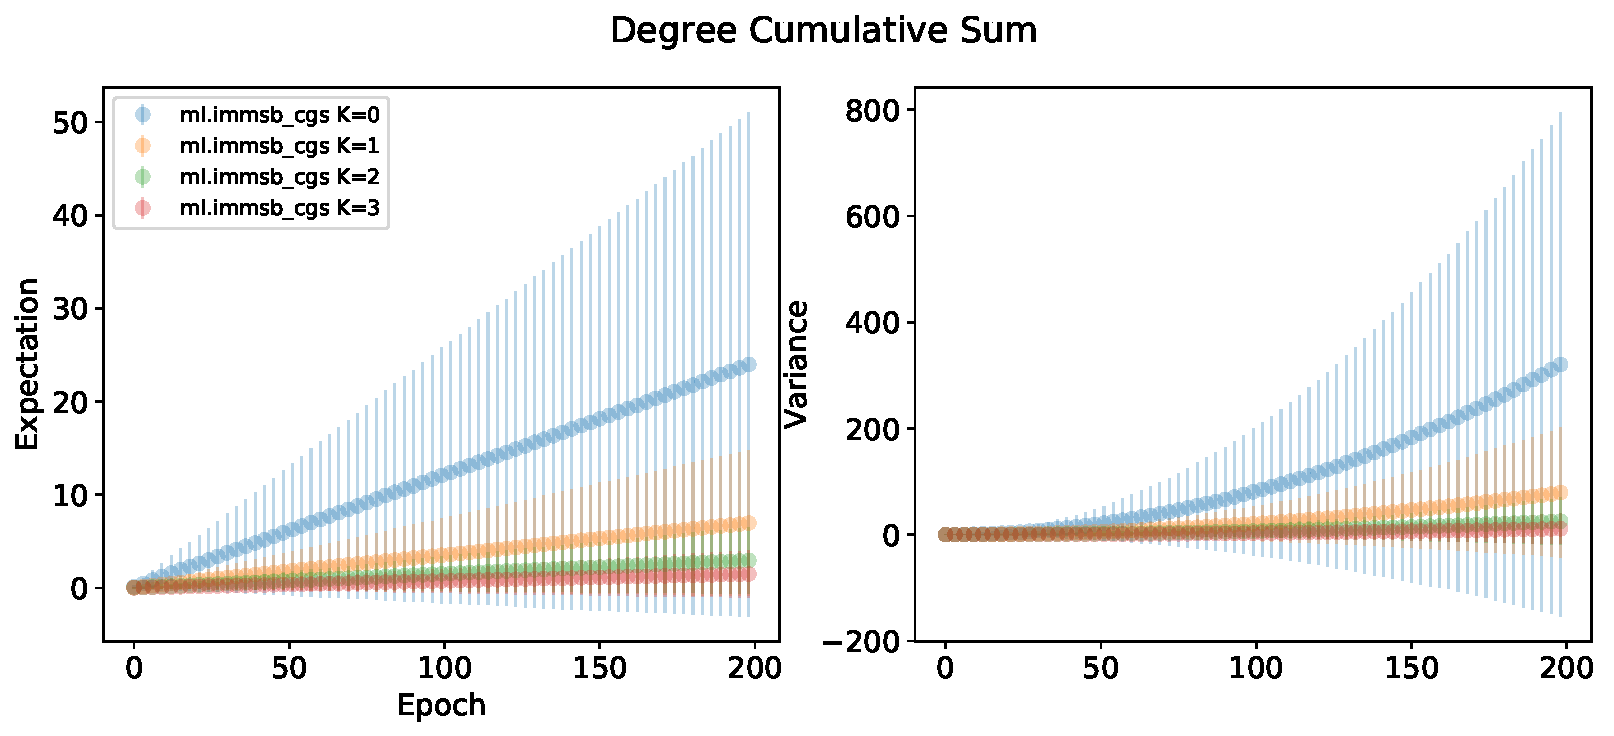
\includegraphics[width=\textwidth]{{{img/0201/ml.immsb_cgs_burst_process_local_mg_ml.immsb_cgs}}}
    \end{minipage}

    \begin{minipage}{0.99\textwidth}
        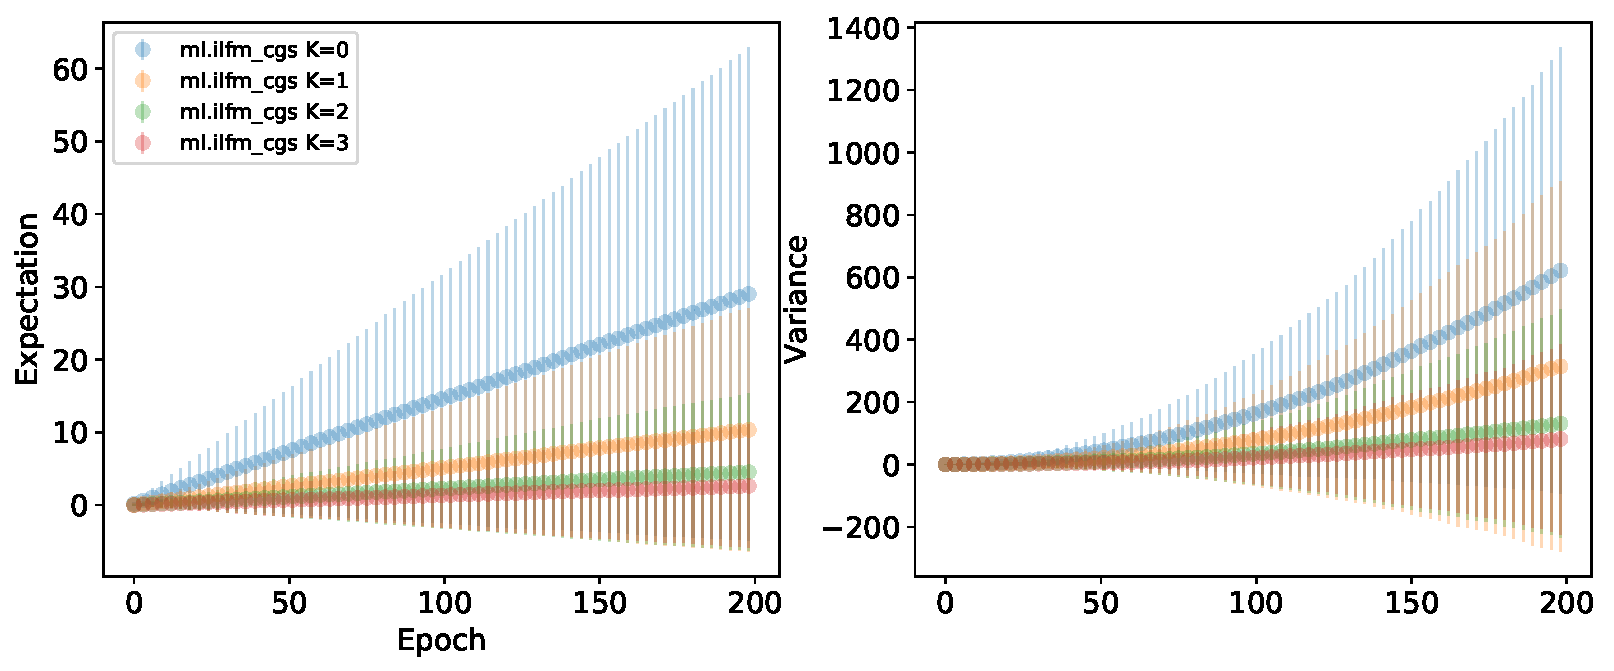
\includegraphics[width=\textwidth]{{{img/0201/ml.ilfm_cgs_burst_process_local_mg_ml.ilfm_cgs}}}
    \end{minipage}
    \caption {Top figure represent IMMSB local degree count process. The left part of the figure is the average overs the network's node and the roght part is the variance. Bottom figure is the same quantities but for ILFM model.} 
\label{fig:mg_deg}
\end{figure}

